\documentclass{scrartcl}
\usepackage[polish]{babel}
\usepackage[utf8]{inputenc}
\usepackage[OT4]{fontenc}
\usepackage{url}
\usepackage{amsmath}
\usepackage{amsfonts}
\usepackage{graphicx}
\usepackage{chngpage}
\usepackage{caption}
\usepackage{subcaption}

\title{Sztuczna inteligencja DAO}
\date{\today}
\author{Tomasz Boczkowski\\ 88189 \and Paweł Lampe\\ 99277}

\begin{document}

\thispagestyle{empty} %bez numeru strony

\begin{center}
{\large{Projekt z laboratorium:\\
Sztucznej Inteligencji na kierunku Informatyka }}

\vspace{3ex}

Implementacja algorytmów sztucznej inteligencji grających w DAO.

\vspace{3ex}
{\footnotesize Poznań,\today}

\end{center}


\vspace{10ex}


\vspace{5ex}

Autorzy:
\begin{tabular}{lllr}
\textbf{Tomasz Boczkowski} & 88189 & I5.1 & tomasz.boczkowski@onet.pl \\
\textbf{Paweł Lampe} & 99277 & I5.1 & pawel.lampe@poczta.fm \\
\end{tabular}

\vspace{5ex}



\newpage



\section{Opis gry}

Gra DAO została opublikowana w 1999 roku. Jej autorami są 
Jeff Pickering i Ben VanBuskirk. Dwa lata później otrzymała ona 
nagrodę \emph{MENSA Select}.

Celem gry Dao jest przesunięcie swoich pionów na jedną z pozycji
wygrywających.

Podczas ruchu, gracz może wykonać ruch każdym ze swoich pionów. Ruch polega na przesunięciu piona w poziomie, w pionie lub na skos. Przesunięcie musi zostać wykonane w danym kierunku aż do napotkania przez dany pion przeszkody. Przeszkodą może być koniec planszy lub pion innego gracza. Zabronione jest przeskakiwanie pionów przeciwnika.

Gracze wykonują swoje ruchy naprzemiennie. 

Początkowy stan gry przedstawiony został na rysunku \ref{fig:begin}.

\begin{figure}[h]
  \centering
  \includegraphics[scale=0.6]{data/position0.pdf}
  \caption{Stan początkowy}
  \label{fig:begin}
\end{figure}

W grze dao wyróżniamy 18 różnych stanów wygrywających:
\begin{itemize}
\item umieszczenie wszystkich swoich pionów w narożnikach planszy.
\item utworzenie w dowolnym miejscu planszy kwadratu 2x2 ze swoich
  pionów (9 takich stanów)
\item utworzenie w dowolnym miejscu planszy linii poziomej lub
  pionowej ze swoich pionów (8 takich stanów)
\end{itemize}

Niedozwolone jest otoczenie pojedynczego piona przeciwnika znajdującego
się w narożniku trzema swoimi pionami. Taka sytuacja oznacza
przegraną otaczającego.

\section{Implementacja}

\subsection{Reprezentacja stanu gry}

Stan gry jest reprezentowany na trzy sposoby. Są one wymienione w
poniższych punktach. Implementacja reprezentacji stanu gry zawarta 
jest w plikach Board.*, State.*.

\subsubsection{Podstawowa reprezentacja macierzowa}

W skład podstawowej reprezentacji stanu gry wchodzi 
macierzowa reprezentacja planszy oraz
wskazanie na gracza wykonującego ruch w bieżącej turze\footnote{
State.h, linie 19-20}. 

Stan planszy reprezentowany jest jako dwuwymiarowa tablica o rozmiarze
4x4\footnote{Board.h, linia 16}. Każdy z jej elementów reprezentuje
pojedyncze pole. Dopuszczalne
wartości elementów tablicy znajdują się w typie wyliczeniowym
\emph{enum FieldState}\footnote{Board.h, linia 4}. Oznaczają one:
\begin{itemize}
\item FIELD\_PLAYER1 - pole, na którym znajduje się pionek gracza 1
\item FIELD\_PLAYER2 - pole, na którym znajduje się pionek gracza 2
\item FIELD\_EMPTY - pole puste
\end{itemize}

Gracza wykonujęcego ruch reprezentuje pojedyncza zmienna typu
\emph{enum FieldState}. Wartości FIELD\_PLAYER1 oraz FIELD\_PLAYER2 
oznaczają odpowiednich graczy, wartość FIELD\_EMPTY nie jest
uzywana.

\subsubsection{Reprezentacja krótka}

Reprezentacja krótka zawiera pełną informację o stanie gry zawartą
w 32--bitowej liczbie całkowitej bez znaku. Jest ona stosowana przy
wykrywaniu cykli. Obliczanie reprezentacji krótkiej zostało
zaimplementowane w metodzie getHash() klasy State\footnote{
State.h, linia 29}.

Stan każdego z 16 pól jest reprezentowany za pomocą dwóch
bitów:
\begin{itemize}
\item $(00)_B$ reprezentuje pole puste
\item $(01)_B$ reprezentuje pole zajęte przez pionek gracza 1
\item $(10)_B$ reprezentuje pole zajęte przez pionek gracza 2
\item $(11)_B$ stan zakazany, przydatny przy rozpoznawaniu kolorów
  graczy.
\end{itemize}

Reprezentacje stanów pól są konkantenowane zgodnie z kolejnością pól
przedstawioną na rysunku \ref{fig:field_order}. Tworzą one 32-bitową
liczbę. Pole numer 16 zajmuje najstarsze bity, pole numer 1 --
najmłodsze. Jeżeli bieżący ruch wykonuje gracz 1,
utworzona liczba jest reprezentacją krótką stanu gry. W przeciwnym
przypadku reprezentacja krótka powstaje 
poprzez zanegowanie bitowe utworzonej w wyniku konkatenacji liczby.

\begin{figure}[h]
  \centering
  \includegraphics{data/field_order.pdf}
  \caption{Kolejność pól przy obliczaniu reprezentacji krótkiej}
  \label{fig:field_order}
\end{figure}

Kolor gracza wykonującego ruch można określić na podstawie
reprezentacji którkiej, wyszukując w
reprezentacji stanu gry sekwencji $(11)_B$. Jest ona obecna wtedy i
tylko wtedy, gracz 2 wykonuje bieżący ruch.

\subsubsection{Reprezentacja krótka niezmienna względem odbić,
  obrotów i kolorów}
Jest to wariant reprezentacji krótkiej. Jest on obliczany w sposób,
zapewniający 
niezmienniczość względem obrotów planszy i odbić lustrzanych w pionie
i poziomie. 

Figury na rysunku \ref{fig:field_order2} zawierają numery pól na
planszy poddanej transformacjom. Dla każdej z 8 transformacji i
określonej przez nią kolejności pól, jest obliczana reprezentacja 
krótka (bez negowania). Spośród obliczonych 8 reprezentacji, 
jest wybierana ta, która stanowi najmniejszą liczbę.

\begin{figure}[h]
  \centering
  \includegraphics[width=\textwidth]{data/field_order2.pdf}
  \caption{Transformacje planszy nie zmieniające stanu gry}
  \label{fig:field_order2}
\end{figure}

Jeżeli gracz 2 wykonuje bieżący ruch, wybrana reprezentacja jest
negowana.

\subsubsection{Przykład}

\paragraph{Reprezentacja macierzowa} Rozważmy stan gry przedstawiony na rysunku \ref{fig:example_state}.
Gracz 2 wykonuje ruch. W podstawowej reprezentacja planszy wygląda
następujaco:

\begin{figure}[h!]
  \centering
  \includegraphics[width=5cm]{data/example_board.pdf}
  \caption{Przykładowy stan gry. Gracz 1 ma kolor czerwony, Gracz 2
niebieski. Gracz 2 wykonuje ruch.}
  \label{fig:example_state}
\end{figure}

\[ \begin{bmatrix}
\text{FIELD\_PLAYER2} & \text{FIELD\_EMPTY} & 
\text{FIELD\_PLAYER1} & \text{FIELD\_PLAYER2} \\ 
\text{FIELD\_EMPTY} & \text{FIELD\_EMPTY} & 
\text{FIELD\_PLAYER1} & \text{FIELD\_EMPTY} \\ 
\text{FIELD\_PLAYER2} & \text{FIELD\_EMPTY} & 
\text{FIELD\_PLAYER2} & \text{FIELD\_PLAYER1} \\ 
\text{FIELD\_EMPTY} & \text{FIELD\_PLAYER1} & 
\text{FIELD\_EMPTY} & \text{FIELD\_EMPTY}
\end{bmatrix}
\]

\paragraph{Reprezentacja krótka} Pierwszym krokiem przy wyliczaniu reprezentacji którkiej jest 
konkatenacja bitowa reprezentacji odpowiednich pól.
\[r = (00\ 00\ 01\ 00\ 01\ 10\ 00\ 10\ 00\ 01\ 00\ 00\ 10\ 01\ 00\ 10
)_B \]
Ponieraż gracz 2 wykonuje ruch, otrzymaną reprezentację należy
zanegować bitowo. Ostatecznie
\[R = ~r = (11\ 11\ 10\ 11\ 10\ 01\ 11\ 01\ 11\ 10\ 11\ 11\ 01\ 10\ 11\ 01)_B
= 4221431698 \]

\paragraph{Reprezentacja krótka niezmienna względem symetrii} Aby obliczyć reprezentację krótką niezmienną względem symetrii planszy
należy wybrać najmniejszą wśród liczb odpowiadających różnym 
kolejnościom pól przedstawionym na rysunku \ref{fig:field_order2}.
\[r_1 = (00\ 00\ 01\ 00\ 01\ 10\ 00\ 10\ 00\ 01\ 00\ 00\ 10\ 01\ 00\ 10
)_B \]
\[r_2 = (10\ 00\ 01\ 00\ 01\ 01\ 10\ 00\ 00\ 00\ 00\ 01\ 10\ 00\ 10\ 00
)_B\]
\[r_3 = (10\ 00\ 01\ 10\ 00\ 00\ 01\ 00\ 10\ 00\ 10\ 01\ 00\ 01\ 00\ 00
)_B\]
\[r_4 = (00\ 10\ 00\ 10\ 01\ 00\ 00\ 00\ 00\ 10\ 01\ 01\ 00\ 01\ 10\ 10
)_B\]
\[r_5 = (00\ 01\ 00\ 00\ 10\ 00\ 10\ 01\ 00\ 00\ 01\ 00\ 10\ 00\ 01\ 10
)_B\]
\[r_6 = (00\ 01\ 00\ 10\ 00\ 10\ 01\ 01\ 01\ 00\ 00\ 00\ 00\ 10\ 00\ 10
)_B\]
\[r_7 = (10\ 00\ 10\ 00\ 00\ 00\ 00\ 01\ 01\ 01\ 10\ 00\ 10\ 00\ 01\ 00
)_B\]
\[r_8 = (10\ 01\ 00\ 10\ 00\ 01\ 00\ 00\ 01\ 10\ 00\ 10\ 00\ 00\ 01\ 00
)_B\]
Wśród wyżej wymienionych liczb najmnjejszą jest:
\[r_1\]
Ponieważ ruch należy do gracza 2, reprezentacja stanu gry powstaje
poprzez zanegowanie $r_1$.
\[R = ~r = (11\ 11\ 10\ 11\ 10\ 01\ 11\ 01\ 11\ 10\ 11\ 11\ 01\ 10\ 11\ 01)_B
= 4221431698 \]

\subsection{Generacja ruchów dopuszczalnych}

Jedynym typem ruchu w grze jest przesunięcie. 
Ruch reprezentowany jest w pamięci komputera jako klasa Move\footnote{
Move.h}. Najważniejsze pola to \emph{from} oraz \emph{to}. Są one
liczbami
całkowitymi. Reprezentują one pola planszy zgodnie z kolejnością 
przedstawioną na rysunku \ref{fig:field_order}. Pole \emph{from}
reprezentuje pole, skąd przesuwany jest pion, a pole \emph{to}
-- pole na które jest przesuwany pionek.

Zbiór ruchów może być przechowywany w strukturze MoveSet\footnote{
Move.h, linia 30}. MoveSet wykorzystuje strukturę listy łączonej
z uprzednio zaalokowaną pamięcią na elementy. Taka implementacja 
umożliwia szybkie wstawianie elementów, filtrowanie, czyszczenie
oraz zmianę konieczności. Jednocześnie unikany jest problem 
wielu alokacji pamięci występujący przy zwykłej liście łączonej.

Generator ruchów dopuszczalnych zaimplementowany jest jako metoda 
klasy \emph{Game} \emph{getAvailableMoves}\footnote{Game.h, linia 28}.
Algorytm wyszukuje pionków bieżącego gracza, iterując po
planszy\footnote{Game.cpp, linie 130-131}. Dla każgego znalezionego
piona, sprawdzana jest możliwość ruchu w każdym z 8 kierunków
(w pionie, poziomie i po skosie)\footnote{Game.cpp, linie 134-139}.
Najpierw sprawdzane są ruchy powodujące przesunięcie w górę 
(górny lewy skos, góra, prawy górny skos). Następnie ruchy nie 
powodujące przesunięcia w pionie (prawo, lewo). Jako ostatnie 
rozpatrywane są ruchy powodujące przesunięcie w dół (dolny lewy
skos, dół, dolny prawy skos).

Generator ruchów tworzy listę wszystkich dostępnych ruchów. Wykrywanie
i usuwanie cykli implementowane jest przez metodę \emph{filterCycles}
klasy \emph{Game}\footnote{Game.h, linia 29, Game.cpp, linie 142-162}.
Metoda ta działa jako filtr dla listy ruchów. 

Kiedy gracz wykonuje ruch, klasa Game zapisuje krótką reprezentację
nowego stanu w zbiorze (klasa std::set) Game::m\_previous\_state\_hashes 
\footnote{Game.cpp, linia 66}.
Przy filtrowaniu cykli obliczane są krótkie reprezentacje stanów gry.
Jeżeli reprezentacja jednego z następników znajduje się w 
Game::m\_previous\_state\_hashes, jest on usuwany.

\begin{figure}[h]
  \centering
  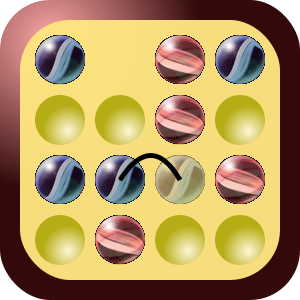
\includegraphics[scale=0.6]{data/example_move.pdf}
  \caption{Przykładowy ruch}
  \label{fig:example_move}
\end{figure}

Przykładowy ruch został przedstawiony na rysunku
\ref{fig:example_move}. Jego reprezentacją jest klasa Move. Jej 
pola mają wartości:
\[\text{from} = 10\]
\[\text{to} = 9\]

\subsection{Metody przeszukiwania stanów gry}

Zaimplementowane zostały dwa algorytmy przeszukiwania stanów gry:
\begin{itemize}
\item $\alpha - \beta$ w wersji klasycznej\footnote{Algorithms.h, 
    linia 29}
\item $\alpha - \beta (\text{failsoft}) + \text{TT}$\footnote{Algorithms.h, linia 73}
\end{itemize}

Algorytm $\alpha - \beta$ został zaimplementowany przy użyciu 
zapisu minimax.

W rekordzie tablicy przejść pamiętane są\footnote{Alhorithms.h, 
linia 63}:
\begin{itemize}
\item{krótka reprezentacja stanu służąca jako klucz}
\item{zapamietana wartość funkcji oceny heurystycznej}
\item{zapamiętane wartości progów alfa, beta}
\item{typ rektordu}
\item{głębokość wierchołka}
\item{najlepszy ruch}
\end{itemize}

Znaczenie tych pól jest identyczne z omówionym na zajęciach 
laboratoryjnych. 

Kluczem tablicy przejść jest reprezentacja krótka stanu niezmienna
względem symetrii omówiona w punkcie 2.1.2. Konflikty różnych 
stanów, pomijając symetryczne, nie występują.

Ze względu na istnienie jednego wpisu w tablicy transpozycji dla
wszystkich symetrycznych stanów gry, należy uwzględnić przekształcenia
najlepszego ruchu. Funkcja \emph{getInvariantHash} klasy \emph{State}
zapisuje numer przekształcenia, które wybrała do obliczenia 
reprezentacji. To samo przekształcenie jest stosowane przy zapisie
ruchu. Przy odczycie ruchu należy zastosować przekształcenie
odwotne. Numer przekształcenia jest wówczas pobierany przy obliczaniu 
klucza.

Ponieważ bicia w grze nie występują, wszystkie wpisy pozostają 
aktualne do końca gry. 
Tablica przejść tworzona jest wraz z początkiem gry.


\subsection{Funkcja oceny heurystycznej stanu gry}

W grze dao wyróżniamy łącznie 22 wszystkie możliwe stany terminalne dla danego gracza:
\begin{itemize}
\item 1 stan - pokrycie narożników
\item 9 stanów - kwadraty 2x2
\item 8 stanów - linie poziome i pionowe
\item 4 stany - blokada przeciwnika w rogu
\end{itemize}
W dalszej części rozważań będziemy używać pojęć które definiuje się następująco:
\begin{itemize}
\item Warstwą będziemy nazywać zbiór stanów terminalnych pokrytych za pomocą odpowiedniej ilości pionów. Tak oto $n$-ta warstwa to zbiór takich stanów terminalnych, że są one kryte przez $n$ pionów danego gracza. Ze względu na powyższe sens mają rzecz jasna tylko warstwy od 1 do 4
\item Przez $r_{n}^{m}$ oznaczać będziemy ilość elementów $n$-tej warstwy dla $m$-tego gracza
\item Przez $p_{n}^{m}$ oznaczać będziemy ilość elementów $n$-tej warstwy dla $m$-tego gracza z pominięciem stanów terminalnych blokowanych przez przeciwnika
\item Przez $k_{n}$ oznaczać będziemy wagę $n$-tej warstwy
\item Przez $h$ oznaczać będziemy współczynnik nadzieji
\item Vetem nazywać będziemy stan terminalny w pełni pokryty
\end{itemize}
Niech dane będą wszelkie wymagane arności. W ogólności możemy wyróżnić następujące wzory:
%equation
$max = 18 ( k_{1} + k_{2} + k_{3} )$
%equation
$h_{n} = p_{1}^{n} k_{1} + p_{2}^{n} k_{2} + p_{3}^{n} k_{3} + h ([r_{1}^{n} - p_{1}^{n}] k_{1} + [r_{2}^{n} - p_{2}^{n}] k_{2} + [r_{3}^{n} - p_{3}^{n}] k_{3})$

$max$ to maksymalna i nieprzekraczalna ocena heurystyczna. Jest to swojego rodzaju przeszacowana górna granica funkcji oceny heurystycznej.

$h_{n}$ to ocena heurystyczna $n$-tego gracza.

$max$ używana jest w sytuacjach veta oraz w sytacji osiągnięcia jednego ze stanów blokady przeciwnika w rogu.

Ostatecznie $h_{n} - h_{1-n}$ to ocena heurystyczna danego stanu.

\section{Testy wydajnościowe i porównania algorytmów}

Dla trzech rożnych stanów poczatkowych dokonano pomiarów liczby
wierzchołków odwiedzonych przez algorytmy $\alpha - \beta$ oraz
$\alpha - \beta + \text{TT}$. Parametry funkcji oceny heurystycznej
przyjmowały wartości $k_1 = 1$, $k_2 = 19$, $k_3 = 131$, $h = 0$.

\begin{figure}[h]
  \centering
  \includegraphics[scale=0.6]{data/position0.pdf}
  \caption{Przykładowy stan gry - stan początkowy}
  \label{fig:position0}
\end{figure}

\begin{table}[h]
  \centering
  \caption{Zestawienie wyników  pomiarów wydajności algorytmów dla stanu
    przedstawionego na rysunku \ref{fig:position0}}
  \label{table:position0}
  \begin{tabular}{|c|c|c|}
\hline
Głębokość &\multicolumn{2}{|c|}{Liczba odwiedzonych wierzchołków}\\
\hline
& $\alpha - \beta$ &$\alpha - \beta + \text{TT}$ \\ 
\hline
5 & 165451 & 35136 \\
\hline
6 & 456523 & 100507 \\
\hline
7 & 3913744 & 505596 \\
\hline
8 & 13590827 & 1359498 \\
\hline
\end{tabular}

\end{table}

\begin{figure}[h]
  \centering
  \includegraphics[scale=0.5]{data/results0.pdf}
  \caption{Zależność liczby odwiedzonych wierzchołków od głębokości
    przeszukiwania dla stanu przedstawionego na rysunku
    \ref{fig:position0}}
  \label{fig:results0}
\end{figure}


\begin{figure}[h]
  \centering
  \includegraphics[scale=0.6]{data/position1.pdf}
  \caption{Przykładowy stan gry}
  \label{fig:position1}
\end{figure}

\begin{table}[h]
  \centering
  \caption{Zestawienie wyników  pomiarów wydajności algorytmów dla stanu
    przedstawionego na rysunku \ref{fig:position1}}
  \label{table:position1}
  \begin{tabular}{|c|c|c|}
\hline
Głębokość &\multicolumn{2}{|c|}{Liczba odwiedzonych wierzchołków}\\
\hline
& $\alpha - \beta$ &$\alpha - \beta + \text{TT}$ \\ 
\hline
5 & 139515 & 71089 \\
\hline
6 & 549378 & 189203 \\
\hline
7 & 3337096 & 714068 \\
\hline
8 & 13610961 & 1589901 \\
\hline
\end{tabular}

\end{table}

\begin{figure}[h]
  \centering
  \includegraphics[scale=0.5]{data/results1.pdf}
  \caption{Zależność liczby odwiedzonych wierzchołków od głębokości
    przeszukiwania dla stanu przedstawionego na rysunku
    \ref{fig:position1}}
  \label{fig:results1}
\end{figure}

\begin{figure}[h]
  \centering
  \includegraphics[scale=0.6]{data/position2.pdf}
  \caption{Przykładowy stan gry}
  \label{fig:position2}
\end{figure}

\begin{table}[h]
  \centering
  \caption{Zestawienie wyników  pomiarów wydajności algorytmów dla stanu
    przedstawionego na rysunku \ref{fig:position2}}
  \label{table:position2}
  \begin{tabular}{|c|c|c|}
\hline
Głębokość &\multicolumn{2}{|c|}{Liczba odwiedzonych wierzchołków}\\
\hline
& $\alpha - \beta$ &$\alpha - \beta + \text{TT}$ \\ 
\hline
5 & 156947 & 78131 \\
\hline
6 & 864731 & 267493 \\
\hline
7 & 3516925 & 842535 \\
\hline
8 & 19280966 & 2423382 \\
\hline
\end{tabular}

\end{table}

\begin{figure}[h]
  \centering
  \includegraphics[scale=0.5]{data/results2.pdf}
  \caption{Zależność liczby odwiedzonych wierzchołków od głębokości
    przeszukiwania dla stanu przedstawionego na rysunku
    \ref{fig:position2}}
  \label{fig:results2}
\end{figure}

\newpage
\clearpage

\section{Wnioski}

Strukturą przeszukiwanej przestrzeni stanów jest graf. Występują w
nim cykle. Szacunkowa liczba stanów oryginalnej wersji gry
(górne ograniczenie) wynosi 900900. Jest to liczba podziałów 
16-elementowego zbioru pół na zbiory 2 zbiory 4-elementowe (piony) i
1 zbiór 8-elementowy (pola puste).

Ze względu na brak możliwości bicia, graf przestrzeni stanów się 
nie zmienia. Branching factor pozostaje stały i wynosi około 11.

Zdecydowanie najlepszą metodą przeszukiwania przestrzeni stanów 
jest algorytm $\alpha - \beta + \text{TT}$. W stosunku do 
,,czystego'' algorytmu $\alpha - \beta$ pozwala on osiągnąć 
90\% redukcję liczby przeszukiwanych wierzchołków.

Wygranie z komputerem jest trudne. Autorom programu nie udało 
do tej pory wygrać z algorytmem $\alpha - \beta$ przy głębokości
przeszukiwania równej 4.

Na tej podstawie można stwierdzić, że heurystyka okazała się
wystarczająca.
\end{document}
